%%%%%%%%%%%%%%%%%%%%%%%%%%%%%%%%%%%%%%%%%
% Bachelor/Master-Arbeit
% Vorlage HTWG EI
%
% Basierend auf
% 
% LaTeX Template
% Version 2.5 (27/8/17)
%
% This template was downloaded from:
% http://www.LaTeXTemplates.com
%
% Version 2.x major modifications by:
% Vel (vel@latextemplates.com)
%
% This template is based on a template by:
% Steve Gunn (http://users.ecs.soton.ac.uk/srg/softwaretools/document/templates/)
% Sunil Patel (http://www.sunilpatel.co.uk/thesis-template/)
%
% Template license:
% CC BY-NC-SA 3.0 (http://creativecommons.org/licenses/by-nc-sa/3.0/)
%
%%%%%%%%%%%%%%%%%%%%%%%%%%%%%%%%%%%%%%%%%

%----------------------------------------------------------------------------------------
%	PACKAGES AND OTHER DOCUMENT CONFIGURATIONS
%----------------------------------------------------------------------------------------

\documentclass[
11pt, % The default document font size, options: 10pt, 11pt, 12pt
%oneside, % Two side (alternating margins) for binding by default, uncomment to switch to one side
ngerman, % english for English
singlespacing, % Single line spacing, alternatives: onehalfspacing or doublespacing
%draft, % Uncomment to enable draft mode (no pictures, no links, overfull hboxes indicated)
%nolistspacing, % If the document is onehalfspacing or doublespacing, uncomment this to set spacing in lists to single
%liststotoc, % Uncomment to add the list of figures/tables/etc to the table of contents
%toctotoc, % Uncomment to add the main table of contents to the table of contents
%parskip, % Uncomment to add space between paragraphs
%nohyperref, % Uncomment to not load the hyperref package
headsepline, % Uncomment to get a line under the header
%chapterinoneline, % Uncomment to place the chapter title next to the number on one line
%consistentlayout, % Uncomment to change the layout of the declaration, abstract and acknowledgements pages to match the default layout
]{MastersDoctoralThesis} % The class file specifying the document structure

\usepackage[utf8]{inputenc} % Required for inputting international characters
\usepackage[T1]{fontenc} % Output font encoding for international characters

\usepackage{mathpazo} % Use the Palatino font by default

\usepackage[backend=bibtex,style=ieee-alphabetic, bibstyle=ieee-alphabetic, maxnames=3,minnames=1,natbib=true]{biblatex} % Use the bibtex backend with the authoryear citation style (which resembles APA)

\addbibresource{example.bib} % The filename of the bibliography

\usepackage[autostyle=true]{csquotes} % Required to generate language-dependent quotes in the bibliography

%----------------------------------------------------------------------------------------
%	MARGIN SETTINGS
%----------------------------------------------------------------------------------------

\geometry{
	paper=a4paper, % Change to letterpaper for US letter
	inner=2.5cm, % Inner margin
	outer=3.8cm, % Outer margin
	bindingoffset=.5cm, % Binding offset
	top=1.5cm, % Top margin
	bottom=1.5cm, % Bottom margin
	%showframe, % Uncomment to show how the type block is set on the page
}

%----------------------------------------------------------------------------------------
%	THESIS INFORMATION
%----------------------------------------------------------------------------------------

\thesistitle{Entwicklung einer KI-basierten Spurerkennung als externe Sensorik} % Todo: Titel aus EI-Portal

\thesistitle{Kamerabasierte Lane-Detection, als Grundlage zur Bewertung von Spurmittenführung/Spurverlassensverhinderung} % Todo: Titel aus EI-Portal
\supervisor{Prof.~Dr.-Ing Christopher Knievel} % Your supervisor's name, this is used in the title page, print it elsewhere with \supname
\supervisors{Dipl. Math. Tom Wagemann}
\examiner{} % Your examiner's name, this is not currently used anywhere in the template, print it elsewhere with \examname
\company{Audi AG} % Name der Firma
\degree{Bachelor of Engineering} % Your degree name, this is used in the title page and abstract, print it elsewhere with \degreename
\author{Tim \textsc{Alkofer}} % Your name, this is used in the title page and abstract, print it elsewhere with \authorname
\addresses{} % Your address, this is not currently used anywhere in the template, print it elsewhere with \addressname

\subject{} % Your subject area, this is not currently used anywhere in the template, print it elsewhere with \subjectname
\keywords{} % Keywords for your thesis, this is not currently used anywhere in the template, print it elsewhere with \keywordnames
\university{Hochschule Konstanz - Technik, Wirtschaft und Gestaltung} % Your university's name and URL, this is used in the title page and abstract, print it elsewhere with \univname

\AtBeginDocument{
\hypersetup{pdftitle=\ttitle} % Set the PDF's title to your title
\hypersetup{pdfauthor=\authorname} % Set the PDF's author to your name
\hypersetup{pdfkeywords=\keywordnames} % Set the PDF's keywords to your keywords
}

\begin{document}

\frontmatter % Use roman page numbering style (i, ii, iii, iv...) for the pre-content pages

\pagestyle{plain} % Default to the plain heading style until the thesis style is called for the body content

%----------------------------------------------------------------------------------------
%	TITLE PAGE
%----------------------------------------------------------------------------------------

\begin{titlepage}
\begin{center}

  \vspace*{.06\textheight}
  \begin{minipage}[t]{\textwidth}
    
\includegraphics[width=0.4\textwidth, keepaspectratio]{Figures/htwg.png}\hspace{0.19\textwidth} 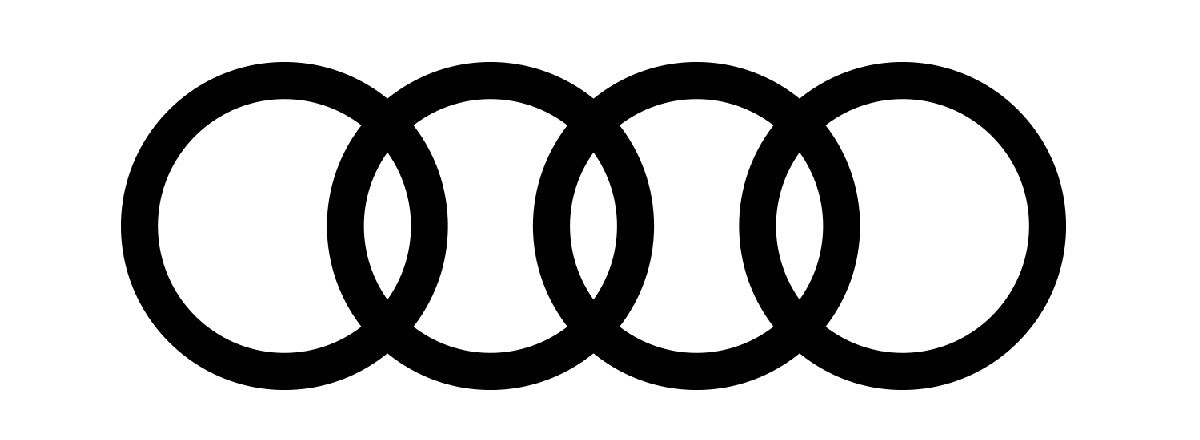
\includegraphics[width=0.4\textwidth,keepaspectratio]{Figures/AL090142_large.jpg}
  \end{minipage}
  {\scshape\LARGE \univname\par\vspace{1em}\supcompany}\vspace{1.5cm} % University name

\HRule \\[0.4cm] % Horizontal line
{\huge \bfseries \ttitle\par}\vspace{0.4cm} % Thesis title
\HRule \\[1.5cm] % Horizontal line

Arbeit zur Erlangung des akademischen Grades: \\[0.4cm]
\textsc{\Large \bfseries \glqq \degreename \grqq}\\[1cm] % Thesis type
absolviert bei der  \\[0.5cm]
\textsc{\Large \bfseries \supcompany}
\\[2cm]
\begin{minipage}[t]{\textwidth}
\begin{flushleft} \large
\emph{Autor:} \authorname % Author name - remove the \href bracket to remove the link
\end{flushleft}
\end{minipage}
\\[1.0cm]
\begin{minipage}[t]{\textwidth}
\begin{flushleft} \large
\emph{1. Prüfer:}
\supname % Supervisor name - remove the \href bracket to remove the link
\\
\emph{2. Prüfer:}
\supnames \\[1cm]
\emph{Eingereicht am:} \today
\end{flushleft}
\end{minipage}\\[3cm]
 
\vfill
\end{center}
\end{titlepage}

%----------------------------------------------------------------------------------------
%	DECLARATION PAGE
%----------------------------------------------------------------------------------------

\begin{declaration}
\addchaptertocentry{\authorshipname} % Add the declaration to the table of contents
\noindent I, \authorname, declare that this thesis titled, \enquote{\ttitle} and the work presented in it are my own. I confirm that:

\begin{itemize} 
\item This work was done wholly or mainly while in candidature for a research degree at this University.
\item Where any part of this thesis has previously been submitted for a degree or any other qualification at this University or any other institution, this has been clearly stated.
\item Where I have consulted the published work of others, this is always clearly attributed.
\item Where I have quoted from the work of others, the source is always given. With the exception of such quotations, this thesis is entirely my own work.
\item I have acknowledged all main sources of help.
\item Where the thesis is based on work done by myself jointly with others, I have made clear exactly what was done by others and what I have contributed myself.\\
\end{itemize}
 
\noindent Signed:\\
\rule[0.5em]{25em}{0.5pt} % This prints a line for the signature
 
\noindent Date:\\
\rule[0.5em]{25em}{0.5pt} % This prints a line to write the date
\end{declaration}

\cleardoublepage


%----------------------------------------------------------------------------------------
%	ACKNOWLEDGEMENTS
%----------------------------------------------------------------------------------------

\begin{acknowledgements}
\addchaptertocentry{\acknowledgementname} % Add the acknowledgements to the table of contents
The acknowledgments and the people to thank go here, don't forget to include your project advisor\ldots
\end{acknowledgements}

%----------------------------------------------------------------------------------------
%	LIST OF CONTENTS/FIGURES/TABLES PAGES
%----------------------------------------------------------------------------------------

\tableofcontents % Prints the main table of contents

\listoffigures % Prints the list of figures

\listoftables % Prints the list of tables

%----------------------------------------------------------------------------------------
%	ABBREVIATIONS
% ----------------------------------------------------------------------------------------

\begin{abbreviations}{ll} % Include a list of abbreviations (a table of two columns)

\textbf{LAH} & \textbf{L}ist \textbf{A}bbreviations \textbf{H}ere\\
\textbf{WSF} & \textbf{W}hat (it) \textbf{S}tands \textbf{F}or\\

\end{abbreviations}

%----------------------------------------------------------------------------------------
%	PHYSICAL CONSTANTS/OTHER DEFINITIONS
%----------------------------------------------------------------------------------------

\begin{constants}{lr@{${}={}$}l} % The list of physical constants is a three column table

% The \SI{}{} command is provided by the siunitx package, see its documentation for instructions on how to use it

Speed of Light & $c_{0}$ & \SI{2.99792458e8}{\meter\per\second} (exact)\\
%Constant Name & $Symbol$ & $Constant Value$ with units\\

\end{constants}

%----------------------------------------------------------------------------------------
%	SYMBOLS
%----------------------------------------------------------------------------------------

\begin{symbols}{lll} % Include a list of Symbols (a three column table)

$a$ & distance & \si{\meter} \\
$P$ & power & \si{\watt} (\si{\joule\per\second}) \\
%Symbol & Name & Unit \\

\addlinespace % Gap to separate the Roman symbols from the Greek

$\omega$ & angular frequency & \si{\radian} \\

\end{symbols}

%----------------------------------------------------------------------------------------
%	DEDICATION
%----------------------------------------------------------------------------------------

\dedicatory{For/Dedicated to/To my\ldots} 

%----------------------------------------------------------------------------------------
%	THESIS CONTENT - CHAPTERS
%----------------------------------------------------------------------------------------

\mainmatter % Begin numeric (1,2,3...) page numbering

\pagestyle{thesis} % Return the page headers back to the "thesis" style

% Include the chapters of the thesis as separate files from the Chapters folder
% Uncomment the lines as you write the chapters

\chapter{Einführung} % Main chapter title

\label{Einführung} 
    Im Rahmen des Studiums Automobilinformationstechnik (B.Eng.) an der HTWG Konstanz gilt es im letzten Semester eine Abschlussarbeit zur Erlangung des akademischen Grades:„Bachelor of Engineering“ zu erstellen. Der vom Verfasser gewählte Betrieb, sowie die ihm zugewiesene Aufgabe sollen im Folgenden näher beschrieben werden.

    \section{Praktikumsbetrieb}
        Die Abschlussarbeit wurde im Zeitraum 01.05.2025 bis 31.07.2025 bei der Audi AG in Ingolstadt erarbeitet. Um ein vollumfängliches Verständnis für das erbrachte Projekt zu vermitteln wird zunächst der Betrieb im Detail vorgestellt.
        \subsection{Historie}
        Nach Spannungen in seinem (1899) zuerst gegründetem Automobilunternehmen Horch \& Cie., baute August Horch 1909 sein zweites Automobilunternehmen, welches seit 1910 als Audiwerke AG arbeitete, in Zwickau auf. Im Jahr 1932 fusionierten dann die vier Marken Audi, DKW, Horch und Wanderer zur Autounion AG. Aus diesem Zusammenschluss resultierte das bis heute bekannte Logo der vier Ringe.
        Nach dem Ende des Zweiten Weltkrieges wurde das Unternehmen enteignet, die Produktionsstätten demontiert und 1948 aus dem Handelsregister der Stadt Chemnitz gelöscht, bis die Autounion AG 1949/1950 mit Sitz in Ingolstadt neu gegründet wurde.
        1969 schlossen sich die NSU AG aus Neckarsulm und die Autounion AG zur Audi NSU Auto Union AG zusammen.
        Seit dem NSU ro 80, der als seiner Zeit (1971) weit voraus galt, ist das Unternehmen für den bis heute genutzten Werbeslogan "Vorsprung durch Technik" bekannt. Diesen technologischen Fortschritt beweiste die Marke beispielsweise durch den ab 1980 im Rallyesport eingesetzten permantenten Allradantrieb quattro, welcher den Sport revolutionierte.
        Seit dem ersten Januar 1985 wird der bis heute genutzte Markenname Audi AG verwendet. \cite{AudiHistory}       
        
        \subsubsection{Konzernstruktur}
        Die Audi AG wurde ab 1964 schrittweise Bestandteil des Volkswagenkonzerns. Der italienische Sportwagenhersteller Lamborghini seit 1998, sowie der Motorradhersteller Ducati seit 2012 gelten wiederum als Audi-Konzerntöchter. Außerdem wechselte der britische Automobilhersteller Bentley ab 2021 von der Markengruppe Sport zu Premium und steht seither ebenfalls unter der Verantwortung der Audi AG. 
        
        Nach eigenen Angaben beschäftigt Audi 2023 mehr als 87.000 Mitarbeiter weltweit. In Ingolstadt befindet sich neben einer Produktionsstätte die Konzernzentrale und die technische Entwicklung, was diesen Standort mit etwa 40.000 Mitarbeitern zum größten des Unternehmens macht.
        Pro Jahr werden hier über 300.000 Fahrzeuge produziert. In Deutschland befinden sich außerdem die Produktionsstandorte Neckarsulm mit etwa 15.000 und Zwickau mit 10.000 Mitarbeitern. Weitere Standorte verteilen sich weltweit unter anderem in Belgien, Ungarn und Mexiko.
        
        Geführt wird die Audi AG aktuell vom Vorstandsvorsitzenden Gernot Döllner. Der Geschäftsbereich Vorsitzender des Vorstands (G) verantwortet wiederum die Geschäftsbereiche Beschaffung (B), technische Entwicklung (E), Finanz, Recht und IT (F), Produktion und Logistik (P), Personal (S) und Marketing und Vertrieb (V). \cite{AudiCompany}

        Unter dem Namen Auto Union GmbH betreibt der Konzern seit 2011 Traditionspflege der Marken: Auto Union, Horch, Audi, DKW, Wanderer und NSU und verantwortet unter anderem das museum mobile in Ingolstadt, sowie den Vertrieb von originalen Ersatzteilen.
        
        Die Audi Sport GmbH ist eine hundertprozentige Tochtergesellschaft der Audi AG. Das Unternehmen wurde 1983 unter dem Namen quattro GmbH gegründet und erlangte 1996 seine Eigenständigkeit, bevor es in Audi Sport GmbH umbenannt wurde. Der Sitz des Unternehmens befindet sich in Neckarsulm. Neben der Verantwortung für die R- und RS-Modelle, betreibt die Audi Sport GmbH vielfältige Projekte im Bereich Motorsport. So wird aktuell an einer eigenen Antriebseinheit für den 2026 anstehenden Einstieg in die FIA Formel 1 gearbeitet.

        
    \section{Einordnung der Abschlussarbeit}
        Die vorliegende Abschlussarbeit wurde in der Organisationseinheit technische Entwicklung absolviert. Das Team der Eigenschaftsteuerung arbeitet innerhalb der Abteilung EX-automatisiertes Fahren/Fahrerassistenz vordergründig an der Objektivierung von subjektiven Eigenschaftswerten bezogen auf Fahrerassistenzsysteme und autonomes Fahren. So wird anhand von Themenspezifischen Fragebögen die subjektive Beurteilung von Testfahrten festgehalten und im Nachhinein den objektiv gemessenen Busgrößen gegenübergestellt, um beispielsweise Kenngrößen für eine sportliche oder komfortable Fahrweise zu ermitteln. Diesen Prozess der Festlegung von messbaren Kenngrößen zu subjektiven Eigenschaften wurde Objektivierung genannt. Aufgeteilt werden dabei die Cluster Fahren, Parken und Safety.

        Eine der Aufgaben des Objektivierungsteams ist Vergleiche zwischen verschiedenen Fahrzeugen und Herstellern zu ziehen. Dazu werden meist Serienfahrzeuge mit eigener Messtechnik ausgestattet, um die Eigenschaften der Fahrerassistenzsysteme zu bewerten. Diese Messtechnik umfasst unter anderem hochgenaue DGPS- und IMU-Sensoren, die eine präzise Positionsbestimmung ermöglichen.
        Somit besteht keine Abhängigkeit zu ggf. verschlüsselten Bus-Daten, die nur für das eigene Fahrzeug verfügbar sind.

        Zur Bewertung von Spurmittenführungssystemen, sowie der Spurverlassensverhinderung innerhalb des Clusters Fahren soll eine externe Sensorik für die Spurerkennung entwickelt werden. Im Detail ist der absolute Abstand zwischen Außenkante des Vorderreifens und Innenkante der Fahrbahnmarkierung als Zielgröße zu ermitteln. Diese Information soll dann in die Objektivierung der Spurmittenführungssysteme einfließen.
        %Todo Skizze/Foto 
    
    \section{Fragestellung}
        Im Rahmen dieser Abschlussarbeit soll eine Sensorik entwickelt werden, die den Abstand zwischen dem Fahrzeug und der Fahrbahnmarkierung ermittelt. Diese Information soll dann in die Objektivierung der Spurmittenführungssysteme einfließen. Die Sensorik soll dabei so konzipiert sein, dass sie an verschiedenen Fahrzeugen eingesetzt werden kann und eine hohe Genauigkeit bei der Messung erreicht wird.
        
        \subsection{Hardware}
        Um die oben genannte Zielgröße zu ermitteln und gleichzeitig Unabhängigkeit, sowie einen einfachen Messaufbau zu gewährleisten, sollen Kameras verwendet werden, die an der Seite des Fahrzeugs montiert werden. Auf dem Kamerabild sollen dann sowohl der Vorderreifen der jeweiligen Fahrzeugseite, sowie der nebenliegende Fahrbahnrand zu erkennen sein.
        So kann dann direkt aus dem relativen Abstand zwischen Fahrbahnmarkierung und Vorderreifen in Pixeln der absolute Abstand in Metern ermittelt werden ohne dabei die relative Position der Kamera zum Fahrzeug zu vermessen zu müssen.
        Für die Umrechnung von Pixeln in Meter wird eine Kalibrierung der Kamera benötigt, die im Rahmen dieser Arbeit mithilfe von Schachbrettmustern durchgeführt wird. Die Kalibrierung soll dabei so gestaltet sein, dass sie auch bei unterschiedlichen Fahrzeugen und Kamerapositionen funktioniert.

        %kalibrierung extrinsisch/intrinsch

%\include{Chapters/Chapter2} 
%\include{Chapters/Chapter3}
%\include{Chapters/Chapter4} 
%\include{Chapters/Chapter5} 

%----------------------------------------------------------------------------------------
%	THESIS CONTENT - APPENDICES
%----------------------------------------------------------------------------------------

\appendix % Cue to tell LaTeX that the following "chapters" are Appendices

% Include the appendices of the thesis as separate files from the Appendices folder
% Uncomment the lines as you write the Appendices

% Appendix A

\chapter{Frequently Asked Questions} % Main appendix title

\label{AppendixA} % For referencing this appendix elsewhere, use \ref{AppendixA}

\section{How do I change the colors of links?}

The color of links can be changed to your liking using:

{\small\verb!\hypersetup{urlcolor=red}!}, or

{\small\verb!\hypersetup{citecolor=green}!}, or

{\small\verb!\hypersetup{allcolor=blue}!}.

\noindent If you want to completely hide the links, you can use:

{\small\verb!\hypersetup{allcolors=.}!}, or even better: 

{\small\verb!\hypersetup{hidelinks}!}.

\noindent If you want to have obvious links in the PDF but not the printed text, use:

{\small\verb!\hypersetup{colorlinks=false}!}.

%\include{Appendices/AppendixB}
%\include{Appendices/AppendixC}

%----------------------------------------------------------------------------------------
%	BIBLIOGRAPHY
%----------------------------------------------------------------------------------------

\printbibliography[heading=bibintoc]

%----------------------------------------------------------------------------------------

\end{document}  

%%% Local Variables:
%%% mode: latex
%%% TeX-master: t
%%% End:
